\section{A Loop Pipeline Algorithm}
\label{sec:pipeline-algo}

We can create a simple certifiable loop pipeline algorithm using the three pipelining primitives. Given a sequential loop $L$ in CCDFG $C$ and pipeline interval $I$, we can create a pipelined loop $L'$ using Algorithm~\ref{algo:disha}. 

Out of these steps, unrolling a loop is a generic compiler transformation. Adding a loop edge is the process of converting an unrolled pipelined loop to a loop which has the back edge in the pipeline full stage to mimic the repetition of the pipeline full stage. Both these steps do not deal with pipelining a loop but merely convert from a loop into its unrolled version and vice versa. We would formalize the proofs of these two steps later. 

\begin{algorithm}[H]
\caption{Certifiable loop pipeline} \label{algo:disha}
\begin{algorithmic}[1]
\Procedure{PipelineLoop}{L, I}
\State $L_1 \leftarrow UnrollLoop (L, I)$.
\State $L_2 \leftarrow \phi-Elimination (L_1) $.
\State $L_3 \leftarrow DataPropagation (L_2) $.
\State $L_4 \leftarrow GenerateShadowRegisters (L_3) $.
\State $ L_5 \leftarrow SuperstepConstruction (L_4) $.
\State $ L' \leftarrow AddLoopEdge (L_5) $.
\State \textbf{return} $(L')$.
\EndProcedure
\end{algorithmic}
\end{algorithm} 

We describe below the steps to convert from an unrolled loop to an unrolled pipelined loop in detail:

\begin{enumerate}
%\item ~Unroll Loop: Unroll loop $L$ by $N / I$ iterations where $N$ is the number of scheduling steps in loop $L$. If the number of scheduling steps is three and pipeline interval is one, we unroll the loop three times. If we pipeline a loop with more that $N / I$ iterations, the pipeline full stage would start repeating.

\item {\bf $\phi$-elimination}: We apply the $\phi$-elimination primitive on an unrolled loop to return a loop in which all the $\phi$-statements have been replaced with their corresponding assignment statements. Figure~\ref{fig:algo1}(a) shows two iterations of the loop for illustration and Figure~\ref{fig:algo1}(b) shows the two iterations after applying the $\phi$-elimination primitive.

\begin{figure}
\begin{center}
\begin{tabular}{ccc}
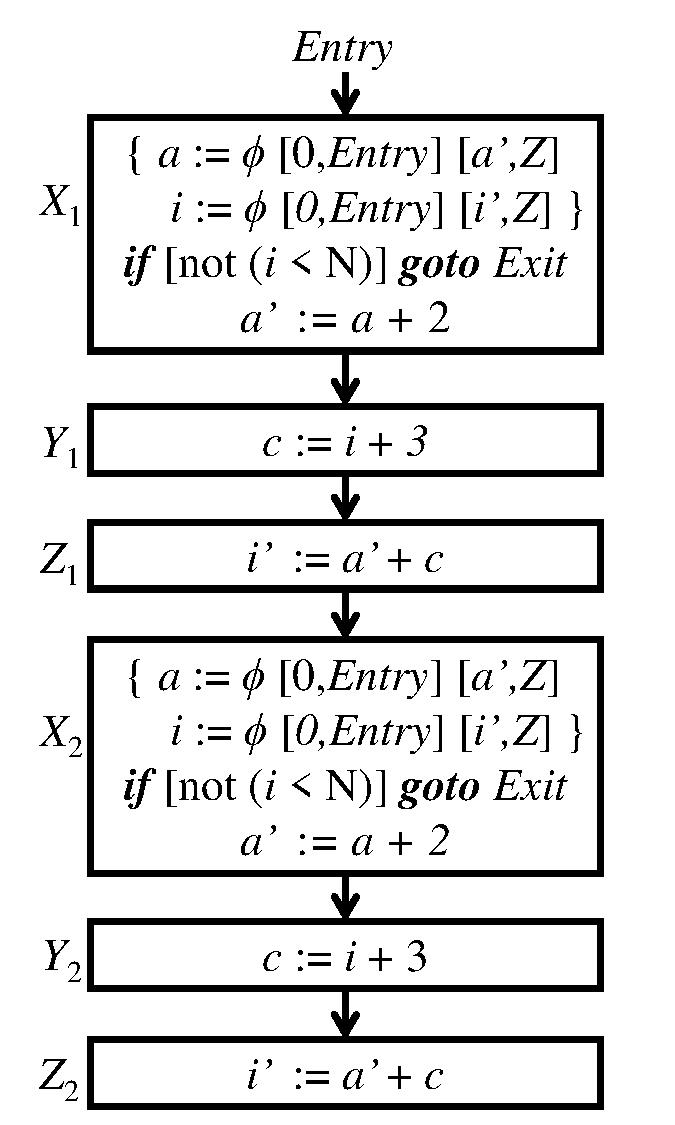
\includegraphics[height=2.5in]{fig-rpe/algorithm-two-iterations}
& 
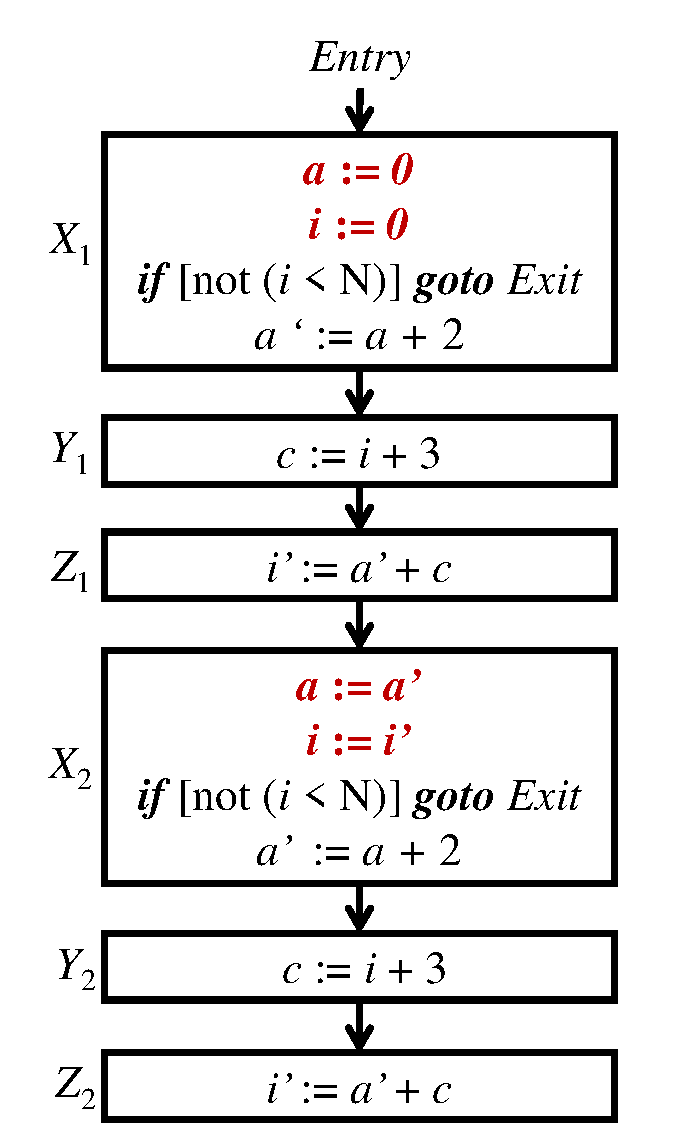
\includegraphics[height=2.5in]{fig-rpe/algorithm-after-phi-elimination}
& 
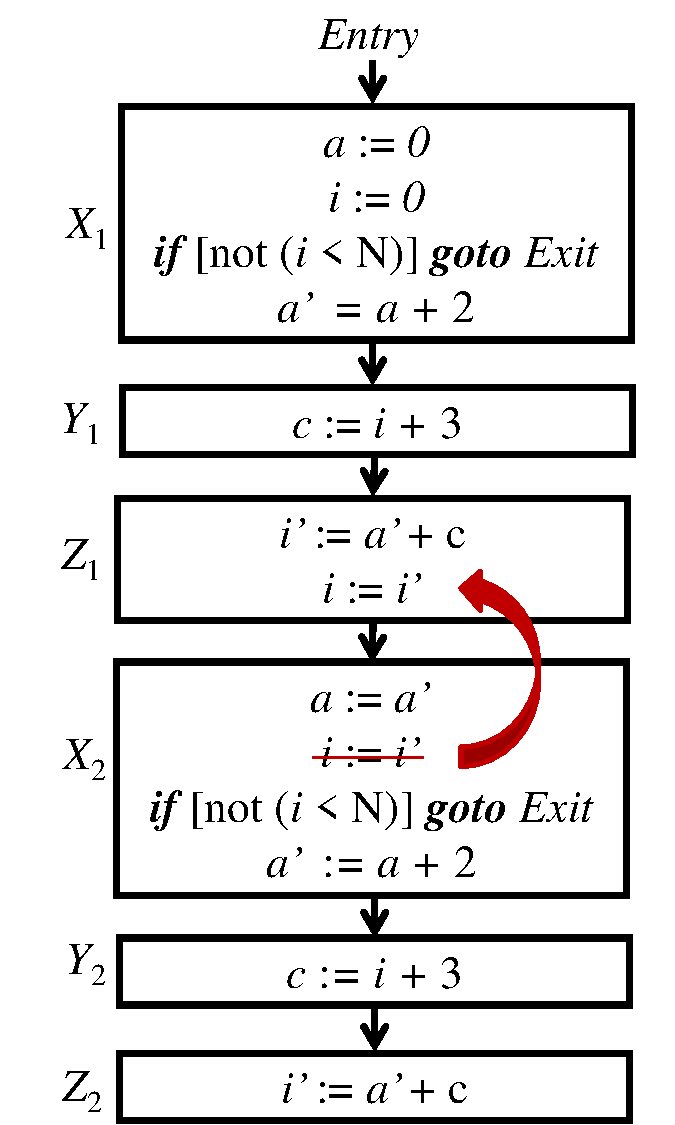
\includegraphics[height=2.5in]{fig-rpe/algorithm-after-data-propagation}
\\
(a) & (b) & (c)
\end{tabular}
\end{center}
\caption{(a) Two iterations of a loop (b) After $\phi$-elimination transformation (c) After data propagation}
\label{fig:algo1}
\end{figure}

\item {\bf Data propagation:} Algorithm~\ref{algo:data-propagation} describes how to compute candidates for data propagation across pipeline iterations. It is a critical step in 


\begin{algorithm}
\caption{Data propagation} \label{algo:data-propagation}
\begin{algorithmic}[1]
\Procedure{DataPropogration}{$L$}
\State $msteps \leftarrow GetLoopCarriedDependencies(L)$.
\For {\textbf{each} mstep \textbf{in} msteps}
 \If {$CheckConflict (L, mstep, N, I) \neq 0$}
\State $L \leftarrow RelocateMStep (L, mstep)$.
\EndIf
\EndFor
\State \textbf{return} $(L)$.
\EndProcedure
\end{algorithmic}
\end{algorithm}

removing data hazards. We want to make sure that when we pipeline a loop, we do not read a variable which has not yet been written. A critical observation is that data propagation is required only for loop carried dependencies.
$GetLoopCarriedDependencies$ identifies the microsteps where loop carried dependencies are being read. Then, $CheckConflict$ checks whether there would be a conflict when we would pipeline the loop. 
%This can be achieved by checking whether the value read in a microstep is written anywhere in the previous $N - I$ \hl{explain} scheduling steps. 
If so, $RelocateMSteps$ relocate the microstep which reads the variable in an iteration to immediately after the microstep which last writes the variable in the previous iteration to remove the conflict. In Figure~\ref{fig:algo1}(c) we found that the loop carried dependency $i'$ in $X_2$ would create a conflict when we would move $X_2$ before $Z_1$ while pipelining. So, we relocate the microstep $i := i'$ after the microstep $i' := a' + c$. Note, $RelocateMStep$ can be seen as an application of a series of interchange primitives. We can only move a microstep upwards till there is no read-write conflict. 

\begin{figure}[t!]
\begin{center}
\begin{tabular}{cc}
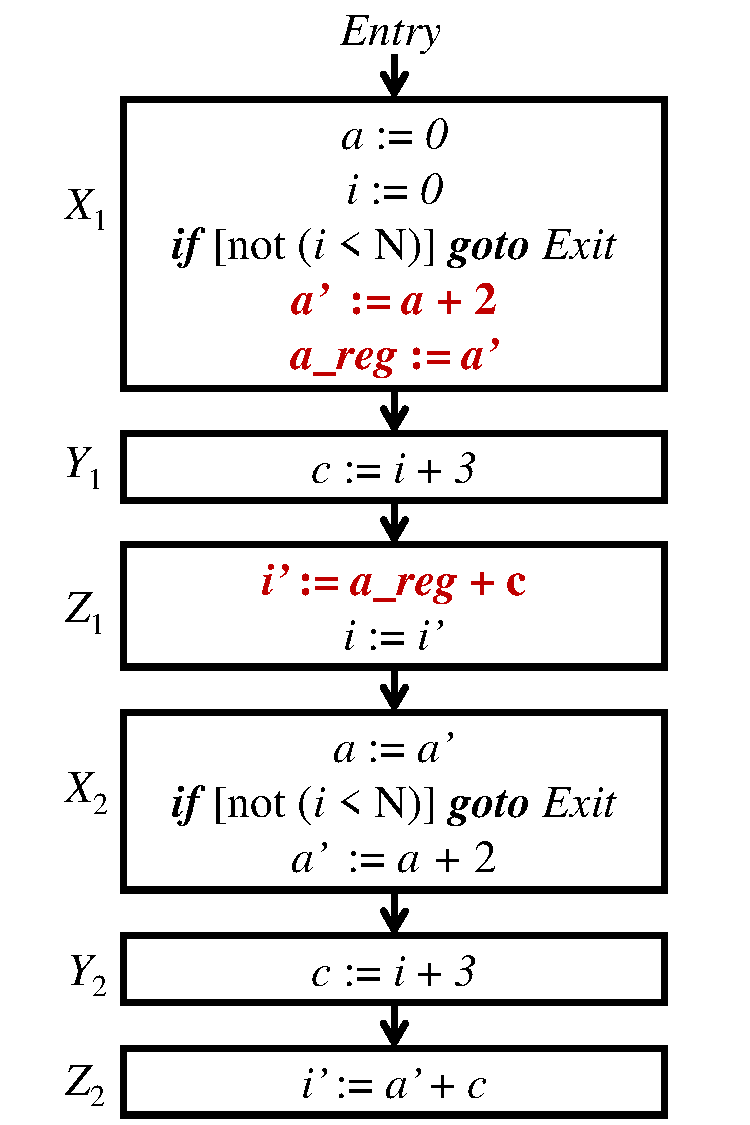
\includegraphics[height=2.5in]{fig-rpe/algorithm-after-shadow-register}
&
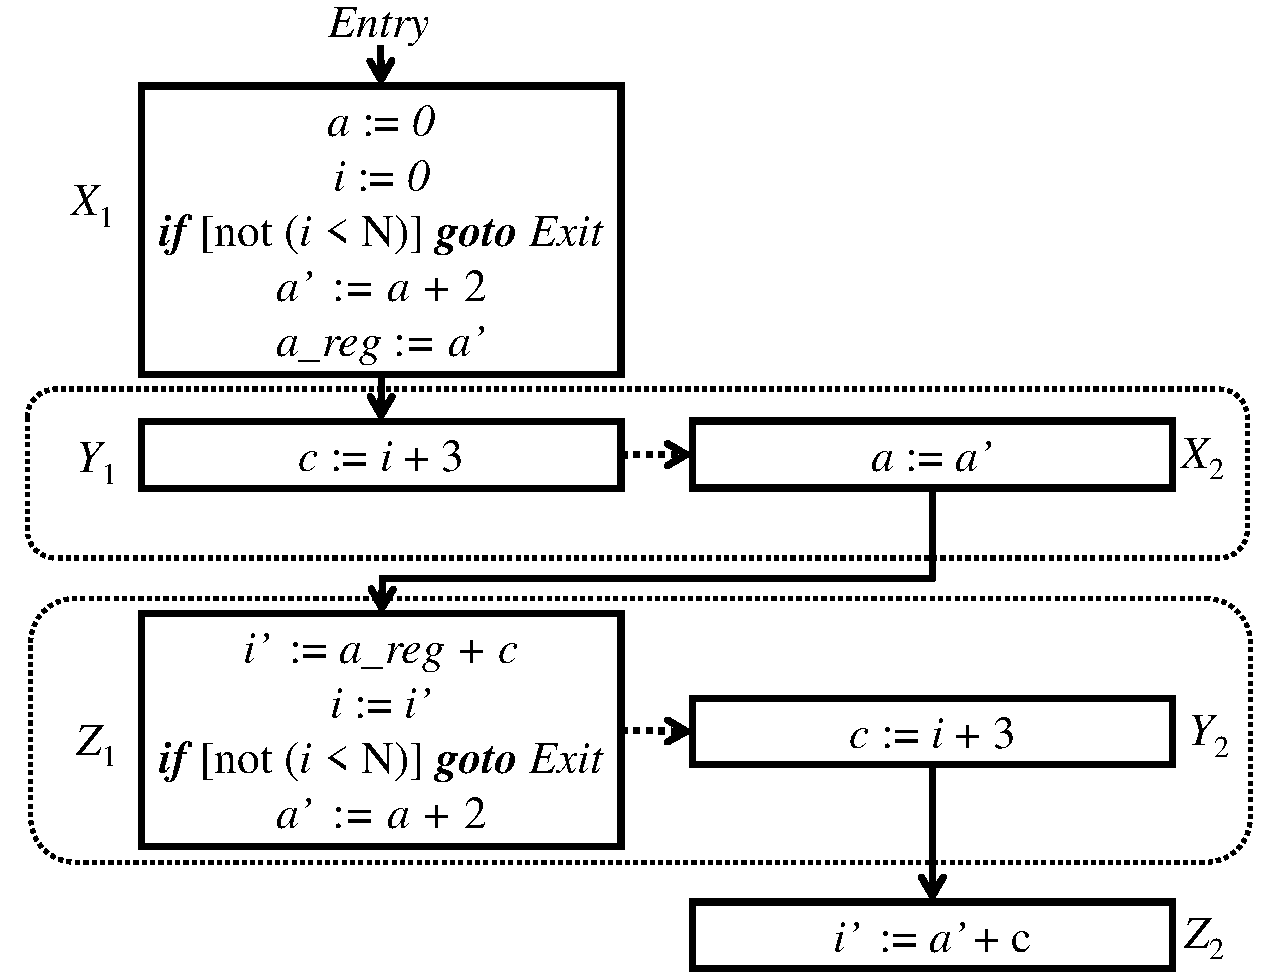
\includegraphics[height=2.5in]{fig-rpe/algorithm-after-superset-construction}
\\
(a) & (b)
\end{tabular}
\end{center}
\caption{(a) After shadow register (b) After superstep construction}
\label{fig:algo2}
\end{figure}

\begin{algorithm}
\caption{Generate shadow registers} \label{algo:generate-pipeline-registers}
\begin{algorithmic}[1]
\Procedure{GenerateShadowRegisters}{$L$}
\State $V \leftarrow GetAllVariables(L)$.
\For {\textbf{each} v \textbf{in} V}
\State $w_v \leftarrow WriteVariable (v, L)$.
\State $r_v \leftarrow LastReadVariable (v, L)$.
%\State $y \leftarrow RequireShadowRegister (r_v, w_v, I)$.
  \If {$RequireShadowRegister (r_v, w_v, I) \neq 0$} 
\State $L \leftarrow AddShadowRegister (w_v, L)$.
\EndIf
\EndFor
\State \textbf{return} $(L)$.
\EndProcedure
\end{algorithmic}
\end{algorithm}

\item {\bf Generate shadow registers:} Algorithm~\ref{algo:generate-pipeline-registers} inserts shadow registers to prevent variables from being overwritten before being read. We first compute all program variables that may be overwritten before being read, which means these are the variables that require shadow registers. To find such variables, $GetAllVariables$ first gets a set of all variables. Then, for each variable, we compare the distance between the write of the variable $w_v$ $(WriteVariable)$ and the last read of the variable $r_v$ $(LastReadVariable)$ in an iteration; if the distance is greater than $I$, %variable is assigned the new data value of the next iteration before current iteration’s value has been fully consumed; this warrants insertion of pipeline variables in every scheduling step between the $r_v$ and $w_v$. The value is propagated every clock cycle following the CCDFG data flow. 
we apply the shadow register primitive on the microstep which writes the variable $(AddShadowRegister)$. We assign that variable to a new variable called shadow register and replace all subsequent reads of that variable with the shadow register till its next write. In Figure~\ref{fig:algo2} (a), we introduce a shadow register $a\_reg$ in iteration 1.
   
\item {\bf Superstep construction:} Now that we have removed the data hazards, we can successfully pipeline the loop using the pipeline interval $I$. We combine the scheduling steps of the successive iterations, forming scheduling ``supersteps'' that act as scheduling steps for the pipelined
implementation. For example, if there are three scheduling steps and the pipeline interval is one, then the unrolled loop structure has nine scheduling steps from ${1 \ldots 9}$. When we pipeline the loop, we have to construct new scheduling steps ${s_1, s_2, \ldots}$ such that $1$ is in $s_1$, $2$ and $4$ are in $s_2$, $3$, $5$ and $7$ are in $s_3$ and so on resembling the pipelined loop structure.
Supersteps must account for read-after-write hazards, i.e, if a variable is written in a scheduling step $s$ and read subsequently in
$s'$ then $s'$ cannot be in a superstep that precedes $s$ in the control/data flow. A scheduling step is allowed to move up another scheduling step only if there are no intermediate read and write conflicts. Note that we implement data forwarding; thus $s$ and $s'$ can be in a single scheduling superstep. 
%Therefore, this step is a  function takes two basic blocks numbers as input, makes sure that there are no read-after-write hazards if we move the second block just before and The result for our example is shown in
%Fig.~\ref{fig:algo2}(b).  
%ConstructSuperstep (x, y) is created by a series of MoveUp operations for each mstep in the scheduling step $x$ such that they reach the position below $y$ if there are no read-write conflicts. 
In Figure~\ref{fig:algo2}(b), scheduling steps $X_2$ and $Z_1$ have no read write conflict now, so we can move step by step the microsteps of $X_2$ using the interchange primitive before $Z_1$. Note, since currently we do not interchange the microstep which has the conditional branch, all the microsteps including and after the conditional branch in $X_2$ do not move above $Z_1$. As part of future work, we would include the conditional branch in the interchange primitive.

%\begin{algorithm}
%\caption{Superstep Construction} \label{algo:superstep-construction}
%\begin{algorithmic}[1]
%\Procedure{SuperstepConstruction}{$L_3$, $N$, $I$}
%\For b 1 to (N - 1)
%\For a 1 to N
%\State $L_3 \leftarrow ConstructSuperstep (a + (N * b), a + (N / I * b))$.
%\State $L_3 \leftarrow ConstructSupersteps (L_3, N, I)$
%\State $L_4 \leftarrow RenameSchedulingSteps (L_4)$.
%\EndFor
%\EndFor
%\State \textbf{return} $(L_4)$.
%\EndProcedure
%\end{algorithmic}
%\end{algorithm}

%\item ~AddLoopEdge --- We add the loop edge (work with Sandip on justification of this step).

\end{enumerate}

It can be seen that the each step in the process to convert an unrolled loop into its pipelined counterpart is a combination of our three primitives. Next, we discuss an outline of the proof of the three primitives using theorem proving.

%\medskip
%\begin{algorithm}
%\caption{Unroll Loop} \label{algo:unroll-loop}
%\begin{algorithmic}[1]
%\Procedure{UnrollLoop}{L, I}
%\State $L_1 \leftarrow \emptyset$.
%\State $N \leftarrow FindNumberOfBlocks (L)$.
%\State $i \leftarrow 0$.
%\While {$i \leq N/I $}
%\State $L_1 \leftarrow AddLoopIteration (L_1)$.
%\State $i \leftarrow i + 1$. 
%\EndWhile 
%\State \textbf{return} $(L_1)$
%\EndProcedure
%\end{algorithmic}
%\end{algorithm}

 